% !Mode:: "TeX:UTF-8"

\chapter{实验设计与分析}
\label{ch:exp}

本章将利用常见的社会关系理解的数据集对上一章提到的PPRN模型进行检测任务的验证,具体来说即对图片中两个标定的坐标人的关系类别。本章首先介绍当前所用到的两个数据集训练/验证/测试的数据分布情况,数据集的特点。再介绍若干对比模型,介绍实验的参数设置,然后分别对实验结果进行说明和分析,并且对其中消息池化进行了不同实现方法的对比。最后通过案例研究的方法来分析PPRN模型在关系补全任务中发挥的效果。

\section{数据集}

\subsection{数据集简介}

现有的大规模社会关系理解的数据集主要有两个:分别是PIPA-relation\cite{sun2017a}数据集和PISC\cite{li2017dual-glance}数据集,下面简单介绍这两个数据集。

PISC数据集全称是People in social Context,它是Sun等人在2017年通过人工标注平台得到的数据集,这些图片主要来自Visual Genome\cite{krishna2017visual}、COCO\cite{lin2014microsoft}、YFCC100M\cite{thomee2016yfcc100m}、instagram 和twitter等社交网站,Google和Bing商业搜索引擎。从这数据额的来源可以保证数据集的图片是足够高的方差的,人的面部表情,以及场景类型。PISC数据集包含22670张图片以及对应的社会关系标注,在PISC数据集上,又包含两个粒度的识别任务,coarse-level和fine-level。如图\ref{fig:exp-pisc-r}所示的划分方式,先是粗粒度的,再到细粒度的关系类别。
\begin{figure}[htpb]
	\centering
	%	\includegraphics[width=0.48 \textwidth, trim=10 10 10 80,clip]{./pic/example_new.pdf}
	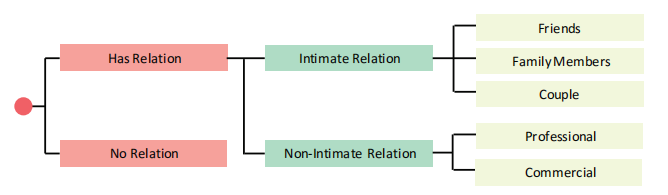
\includegraphics[width=0.98 \textwidth,clip]{pisc-split.png}
	%\hspace{0.02\textwidth}
	%\vspace*{-0.08cm}
    \caption{PISC的关系划分}
	\vspace*{-3.5mm}
	\label{fig:exp-pisc-r}
\end{figure}

PIPA-relation数据集的全称是People in Photo Album Relation,总共包括37107张图片。同样是人工标注的数据集,基于社会关系理论\cite{bugental2000acquisition}划分的,Sun\cite{sun2017a}详细的给出了每个关系域的特征。然后所有的社会关系划分为5个关系域,在构建数据集的过程中,这5个关系域划分为16种社会关系,五个关系域分别是Attachment domain、Reciprocity domain、Mating domain、Hierarchical power domain和Coalitional groups domain。Attach domain划分为father-child,mother-child,Grandpa-grandchild和grandma-grandchild,Reciprocity domain划分为friends, siblings和classmates。Mating domain只包含单条关系lovers/spouses。Hierarchical power domain划分为presenter-audience, teacher-student, trainer-trainee and leader-subordinate。Coalitional groups domain划分为band members, dance team members, sport team members and colleagues。

数据集的情况如表\ref{tab:exp-sta-one},``Train''表示训练集图片的数量,``Valid''和``Test''分别表示验证和测试集的图片数量。``\#train''表示训练集人对的数量,``\#valid''和``\#test''分别表示验证和测试集的人对数量。
\begin{table}[htpb]
  \centering
  \caption{PISC、PIPA-relation数据集的统计表1}
  \label{tab:exp-sta-one}
  \setlength{\tabcolsep}{4.5mm}
  \begin{tabular}{c|c|c|c|c|c|c}
    \toprule
    数据集 & Train & Valid & Test & \#train  &  \#valid &  \#test  \\
    \midrule
    PISC-coarse & 13142 & 4000 & 4000 & 14536 & 25636 & 15497   \\
    \midrule
    PISC-fine &  16828 & 500 & 1250 & 55400 & 1505 & 3691 \\
    \midrule
    PIPA-relation & 5857 & 261 & 2452 & 13729 & 709 & 5106 \\
    \bottomrule
  \end{tabular}
\end{table}

\subsection{数据集分析}

对于数据集PISC-coarse、PISC-fine和PIPA-relation,本文做了基本的数据集分析,如表\ref{tab:exp-sta-two},其中``Sui''表示一张图片有多个人对的比例,``Unsui''则表示一张图片只有一个人对的百分比。·``Single Rel''一张图片包含的关系类别只有一种,``Multi Rel''表示一张图片包含多种关系。从表统计数据可以得到两个结论,从``Sui''和``Unsui''来看,绝大多数的图片是包含多个人对的,从``Multi Rel''来看,一张图片的关系种类往往是相同的,因为直观来看,给定场景下的社会关系时稳定的。例如,假如张图片是一个会议的场景,那么其中往往会有多个人对,并且这些人对间的社会关系往往是``
colleagues''或``presenter audience''。
\begin{table}[htpb]
  \centering
  \caption{PISC、PIPA-relation分析表}
  \label{tab:exp-sta-two}
  \begin{tabular}{c|c|c|c|c}
    \toprule
    数据集 & Sui. & Unsui. & Single Rel & Multi Rel \\
    \midrule
    PISC-coarse  & 87.1 & 12.9 & 79.9 & 20.1 \\
    \midrule
    PISC-fine  & 83.9 & 16.1 & 86.4 & 13.6 \\
    \midrule
    PIPA-relation & 71.9 & 28.1 & 94.9 & 5.1 \\
    \bottomrule
  \end{tabular}
\end{table}

此外,对于关系类别这项统计,本文做了进一步工作,并且发现一张图片的关系种类大多只是一种,少部分是两种。如图\ref{fig:exp-statistic}所示,在PISC-coarse中,大约79.9\%的图片是只有一种关系类别,20.0\%的图片有含有两个关系。

\begin{figure}[htpb]
	\centering
	%	\includegraphics[width=0.48 \textwidth, trim=10 10 10 80,clip]{./pic/example_new.pdf}
	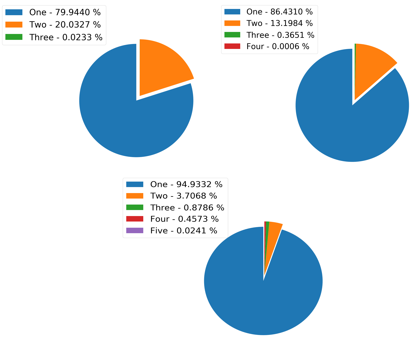
\includegraphics[width=0.65 \textwidth,clip]{ppp.png}
	%\hspace{0.02\textwidth}
	%\vspace*{-0.08cm}
    \caption{数据集的关系类别统计}
	\vspace*{-3.5mm}
	\label{fig:exp-statistic}
\end{figure}

\section{实验设置}

在预训练模型,包括ResNet-101和Vgg-16最后一层的维度都是是4096,经过全连接层,在消息传递和池化模块的中的编码长度为512。结合周边物体信息模块中注意力机制的attention\_size=30,在微调ResNet-101和Vgg-16,卷积层学习率设置为$1 \times 10^{-4}$,新增的分类层学习率为$1 \times 10^{-3}$。训练时,学习率设置为$1 \times 10^{-4}$,权重衰减为$5 \times 10^{-4}$。消息传递和池化模块的迭代数$T=4$。 并且微调时的优化方法是SGD,训练迭代模块的优化方法是Adam。

\subsection{PISC数据集对比}
在实验中,本文主要与以下几个模型进行对照:
\begin{itemize}
    \item \textbf{UnionCNN}学习Lu等人\cite{lu2016visual}利用一个CNN网络来预测关系方法,同样利用一个CNN网络来提取人对的联合区域的特征来进行分类任务。
    \item \textbf{Pair CNN}\cite{li2017dual-glance}由两个共享参数的CNNs提取两个修剪出来的图像特征进行分类。
    \item \textbf{Pair CNN + BBox + Union}\cite{li2017dual-glance}在前面两个特征提取模块的基础上,进一步结合两个个体包围盒的位置信息。
    \item \textbf{Dual-glance}\cite{li2017dual-glance}实现两个粒度的分类任务,分别是PISC-coarse和PISC-fine,分别包含三种和6中类别的关系。Dual-glance利用了PairCNN+BBox+Union,以及物体区域的特征来提存预测结果。
    \item GRM\cite{wang2018deep}提出了一个图推理模型来促进社会关系理解,该模型集成物体和社会关系共现概率的先验知识,GRM采用的是人对特征和上下文物体特征之间的消息传递。
\end{itemize}

类似于GRM模型,我们采用的是每个类别的召回率和mAP(mean average precision)。mAP常作为物体检测的衡量标准,它是不同召回值的下最大精度的平均值。举例如下,假设当前图片有五个苹果,首先对物体检测模型所有检测框分类的类别为苹果按得分从大到小排序。依次计算准确率和召回率,这里的准确率指的是TP和FP。假如总共有10个检测框被识别为苹果,其计算结果如表格\ref{tab:exp:map}所示,例如其中的对于排名第三的降本,$\textbf{Precision} = 2/3 = 0.67$,$\textbf{Recall} = 2/5 = 0.4$。
\begin{table}[htpb]
  \centering
  \caption{mAP计算示例数据}
  \label{tab:exp-map}
  \begin{tabular}{c|c|c|c|c|c|c|c}
    \toprule
    \textbf{得分排名} & \textbf{correct?} & \textbf{Precision} & \textbf{Recall}  & \textbf{得分排名} & \textbf{correct?} & \textbf{Precision} & \textbf{Recall}   \\
    \midrule
    1 & True & 1.0 & 0.2  & 6 & True & 0.5 & 0.6    \\
    \midrule
    2 &  True & 1.0 & 0.4  & 7 & True & 0.57 & 0.8  \\
    \midrule
    3 & False & 0.67 & 0.4  & 8 & False & 0.5 & 0.8  \\
    \midrule
    4 & False & 0.5 & 0.4   & 9 & False & 0.44 & 0.8 \\
    \midrule
    5 & False & 0.4 & 0.4  & 10 & True & 0.5 & 1.0 \\
    \bottomrule
  \end{tabular}
\end{table}
根据数据,以Recall为横坐标,Precision为纵坐标,可以画出如图\ref{fig:exp-map}所示的曲线c。将recall值划分为11个值,我们将$Recall \geq \widetilde{r}$的Precision替换为最大的,由此可得到曲线c。计算方法如公式
\ref{eq:exp-map}所示。我们给定的数据,对于苹果这一类别的AP = $(5 \times 1.0 + 4 \times 0.57 + 2 \times 0.5)/11$
\begin{figure}[htpb]
	\centering
	%	\includegraphics[width=0.48 \textwidth, trim=10 10 10 80,clip]{./pic/example_new.pdf}
	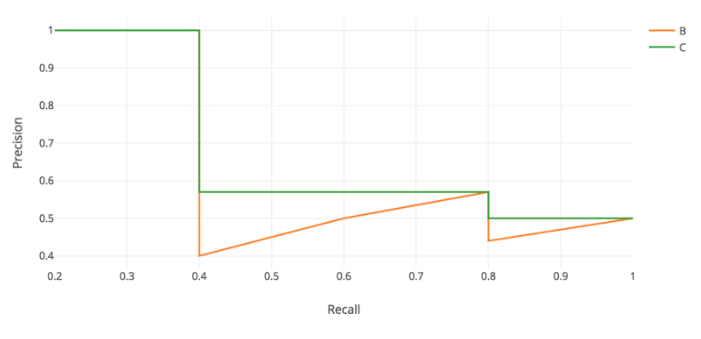
\includegraphics[width=0.75 \textwidth,clip]{map.png}
	%\hspace{0.02\textwidth}
	%\vspace*{-0.08cm}
    \caption{mAP计算示例图}
	\vspace*{-3.5mm}
	\label{fig:exp-map}
\end{figure}
\begin{equation} \label{eq:exp-map}
\begin{split}
    \mathbf{AP} = \frac{1}{11}\sum_{r \in \{0.0,0.1....,1.0\}}P_{interp}(r) \\
    \mathbf{P}_{intern}(r) = max_{\widetilde{r} \geq r}p(\widetilde{r})
\end{split}
\end{equation}

\subsection{PIPA-relation数据集对比}

\section{实验分析}


